\documentclass[bluish,slideColor,colorBG,pdf]{prosper}
\hypersetup{pdfpagemode=FullScreen}
\usepackage{graphicx,amsfonts,amsmath}
\def\baselinestretch{1.0}
\setlength{\topmargin}{-60pt}
\setlength{\textheight}{460pt}
\setlength{\oddsidemargin}{0pt}
\setlength{\evensidemargin}{0pt}
\setlength{\textwidth}{660pt}
\setlength{\footskip}{0pt}
\parindent 0.3in
\hyphenpenalty=10000
\tolerance=10000
\pagestyle{empty}

\def\Prob{{\rm Prob\;}}
\def\prob{{\rm \;Prob\;}}
\def\Var{{\rm Var}}        % Var
\def\Cov{{\rm Cov}}        % Cov

\DeclareSymbolFont{AMSb}{U}{msb}{m}{n}
\DeclareMathSymbol{\expect}{\mathalpha}{AMSb}{'105}

% bold math (use \bm{...})
\def\bm#1{\mathpalette\bmstyle{#1}}
\def\bmstyle#1#2{\mbox{\boldmath$#1#2$}}

\title{Week 9a: coalescents}
\author{Genome 562}
\institution{March, 2017}

\begin{document}

\maketitle

% \begin{slide}[Replace]{The Wright-Fisher model}
% \bigskip
% 
% This is the canonical model of genetic drift in populations.  It was
% invented in 1930 and 1932 by Sewall Wright and R. A. Fisher.
% \bigskip
% 
% In this model the next generation is produced by doing this:
% \begin{itemize}
% \setlength{\itemsep}{5pt}
% \item Choose two individuals {\it with replacement} (including the
% possibility that they are the same individual) to be parents,
% \item Each produces one gamete, these become a diploid individual,
% \item Repeat these steps until $\mathsf{N}$ diploid individuals have been
% produced.
% \end{itemize}
% 
% The effect of this is to have each locus in an individual in the next generation
% consist of two genes sampled from the parents' generation at random,
% with replacement.
% 
% \end{slide}

\begin{slide}[Replace]{Gene copies in a population of 10 individuals }

\vspace{-0.2in}

\centerline{\includegraphics[width=3.2in]{coal1-0.ydraw}}

\end{slide}

\begin{slide}[Replace]{Going back one generation}

\vspace{-0.2in}

\centerline{\includegraphics[width=3.2in]{coal1-1.ydraw}}

\end{slide}

\begin{slide}[Replace]{ ... and one more}

\vspace{-0.2in}

\centerline{\includegraphics[width=3.2in]{coal1-2.ydraw}}

\end{slide}

\begin{slide}[Replace]{ ... and one more}

\vspace{-0.2in}

\centerline{\includegraphics[width=3.2in]{coal1-3.ydraw}}

\end{slide}

\begin{slide}[Replace]{ ... and one more}

\vspace{-0.2in}

\centerline{\includegraphics[width=3.2in]{coal1-4.ydraw}}

\end{slide}

\begin{slide}[Replace]{ ... and one more}

\vspace{-0.2in}

\centerline{\includegraphics[width=3.2in]{coal1-5.ydraw}}

\end{slide}

\begin{slide}[Replace]{ ... and one more}

\vspace{-0.2in}

\centerline{\includegraphics[width=3.2in]{coal1-6.ydraw}}

\end{slide}

\begin{slide}[Replace]{ ... and one more}

\vspace{-0.2in}

\centerline{\includegraphics[width=3.2in]{coal1-7.ydraw}}

\end{slide}

\begin{slide}[Replace]{ ... and one more}

\vspace{-0.2in}

\centerline{\includegraphics[width=3.2in]{coal1-8.ydraw}}

\end{slide}

\begin{slide}[Replace]{ ... and one more}

\vspace{-0.2in}

\centerline{\includegraphics[width=3.2in]{coal1-9.ydraw}}

\end{slide}

\begin{slide}[Replace]{ ... and one more}

\vspace{-0.2in}

\centerline{\includegraphics[width=3.2in]{coal1-10.ydraw}}

\end{slide}

\begin{slide}[Replace]{ ... and one more}

\vspace{-0.2in}

\centerline{\includegraphics[width=3.2in]{coal1-11.ydraw}}

\end{slide}

\begin{slide}[Replace]{The genealogy of gene copies is a tree}

\centerline{\includegraphics[height=3in]{coalgenes.ydraw}}

\end{slide}

\begin{slide}[Replace]{Ancestry of a sample of 3 copies}

\centerline{\includegraphics[height=3in]{coalthree.ydraw}}

\end{slide}

\begin{slide}[Replace]{Here is that tree of 3 copies in the pedigree}

\centerline{\includegraphics[height=3in]{coalinped.ydraw}}

\end{slide}

\begin{slide}[Replace]{Sir John Kingman}

\centerline{\includegraphics[height=2in]{kingman3.ps}}
\bigskip

\centerline{J. F. C. Kingman in about 1983}
\bigskip

Currently Emeritus Professor of Mathematics at Cambridge University,
U.K., and former head of the Isaac Newton Institute of Mathematical
Sciences.

\end{slide}

\begin{slide}[Replace]{Kingman's coalescent}

\centerline{\includegraphics[height=2.2in]{kingman3.ydraw}}
\bigskip

What's misleading about this diagram: the lineages that coalesce are random
pairs, not necessarily ones that are next to each other in a linear order.

\end{slide}

\begin{slide}[Replace]{The coalescent -- a derivation}
\bigskip

The probability that $~\mathsf{k}~$ lineages becomes $~\mathsf{k-1}~$ one generation
earlier turns out to be (as each lineage ``chooses'' its ancestor independently):
\[
\mathsf{k(k-1)/2 \times \Prob({\rm First~two~have~same~parent,~rest~are~different})}
\]
(since there are $~\mathsf{{k \choose 2} = k(k-1)/2}~$ different pairs of copies)

We add up terms, all the same, for the $~\mathsf{k(k-1)/2}~$ pairs that
could coalesce; the sum is:
\[
\begin{array}{r}
\mathsf{k(k-1)/2\;\times\;1\;\times\;\frac{1}{2N}\;\times\;\left(1 - \frac{1}{2N}\right)}
\\\\
\mathsf{\ \ \ \times\;\left(1 - \frac{2}{2N}\right)\;\times\dots
\times\;\left(1 - \frac{k-2}{2N}\right)}
\end{array}
\]
so that the total probability that a pair coalesces is
\[
\mathsf{=\  k(k-1)/4N + O(1/N^2)}
\]

\end{slide}

\begin{slide}[Replace]{Probabilities of two or more lineages coalescing}

Note that the total probability that some combination of lineages
coalesces is
\[
\mathsf{1 - \Prob({\rm Probability~all~genes~have~separate~ancestors})}
\]

\[
\mathsf{=\ 1 - \left[\ 1 \times \left(1 - \frac{1}{2N}\right) \left(1 - \frac{2}{2N}\right) \dots \left(1 - \frac{k-1}{2N}\right)\right]}
\]

\[
\mathsf{=\ 1\ -\ \left[\ 1\ -\ \frac{1+2+3+\dots+(k-1)}{2N}\ +\ O(1/N^2)\ \right]}
\]
and since
\[
\mathsf{1\ +\ 2\ +\ 3\ +\ \dots\ +\ (n-1) \ = \ n(n-1)/2}
\]
the quantity
\[
\mathsf{= \ 1\ -\ \left[\ 1 - k(k-1)/4N + O(1/N^2)\right] \ \simeq \ k(k-1)/4N\ + \ O(1/N^2)}
\]

\end{slide}

\begin{slide}[Replace]{Can calculate how many coalescences are of pairs}
\bigskip

This shows, since the terms of order $\mathsf{~1/N~}$ are the same,
that the events involving 3 or more lineages simultaneously
coalescing are in the terms of order $~\mathsf{1/N^2}~$ and thus become unimportant
if $~\mathsf{N}~$ is large.
\bigskip

Here are the probabilities of 0, 1, or more coalescences with 10 lineages
in populations of different sizes:
\bigskip

\begin{center}
\begin{tabular}{c | c c c}
$\mathsf{N}$ & 0 & 1 & $>1$\\
\hline
\raisebox{3pt}{\strut}100 &  0.79560747  & 0.18744678  &  0.01694575\\
1000 &  0.97771632  &   0.02209806  &   0.00018562\\
10000 & 0.99775217  &  0.00224595  & 0.00000187\\
\end{tabular}
\end{center}
\bigskip

Note that increasing the population size by a factor of 10 reduces the
coalescent rate for pairs by about 10-fold, but reduces the rate for
triples (or more) by about 100-fold.

\end{slide}

\begin{slide}[Replace]{The coalescent}

To simulate a random genealogy, do the following:
\begin{enumerate}
\item Start with $~\mathsf{k}~$ lineages
\item Draw an exponential time interval with mean $\mathsf{~4N/(k(k-1))}~$ generations.
\item Combine two randomly chosen lineages.
\item Decrease $~\mathsf{k}~$ by 1.
\item If $\mathsf{~k = 1}$, then stop
\item Otherwise go back to step 2.
\end{enumerate}

\end{slide}

\begin{slide}[Replace]{How deep is the common ancestor? }
\bigskip

Take expected sizes of coalescents with $\mathsf{n}$, $\mathsf{n-1}$, ... lineages down to 2.
\bigskip

\[
\mathsf{4N \times \left(\frac{1}{n(n-1)} \right) \ = \ 4N \times \left(\frac{1}{n-1} -
\frac{1}{n}\right)}
\]

\[
\mathsf{4N \times \left(\frac{1}{(n-1)(n-2)} \right) \ = \ 4N \times \left(\frac{1}{n-2} -
\frac{1}{n-1}\right)}
\]

\noindent
and so on until 2:

\[
\mathsf{4N \times \left(\frac{1}{2 \times 1} \right) \ = \ 4N \times \left(\frac{1}{1} -
\frac{1}{2}\right)}
\]

\noindent
and cancelling lots of terms in the sum of these

\[
\mathsf{4N \left(1 - \frac{1}{n}\right)}
\]

\end{slide}

\begin{slide}[Replace]{An accurate analogy: Bugs In A Box}

\parbox[b]{1.5in}{There is a box ... \\ \\ \\ \\ \\ \\ } \hspace{0.3in}
\includegraphics[width=2.5in]{bugbox1.idraw}

\end{slide}

\begin{slide}[Replace]{An accurate analogy: Bugs In A Box}

\parbox[b]{1.5in}{with bugs that are ...\\ \\ \\ \\ \\ \\ \\ } \hspace{0.3in}
\includegraphics[width=2.5in]{bugbox2.idraw}

\end{slide}

\begin{slide}[Replace]{An accurate analogy: Bugs In A Box}

\parbox[b]{1.5in}{hyperactive, ...\\ \\ \\ \\ \\ \\ \\ } \hspace{0.3in}
\includegraphics[width=2.5in]{bugbox3.idraw}

\end{slide}

\begin{slide}[Replace]{An accurate analogy: Bugs In A Box}

\parbox[b]{1.5in}{indiscriminate, ...\\ \\ \\ \\ \\ \\ \\ } \hspace{0.3in}
\includegraphics[width=2.5in]{bugbox5.idraw}

\end{slide}

\begin{slide}[Replace]{An accurate analogy: Bugs In A Box}

\parbox[b]{1.5in}{voracious ...\\ \\ \\ \\ \\ \\ \\ } \hspace{0.3in}
\includegraphics[width=2.5in]{bugbox6.idraw}

\end{slide}

\begin{slide}[Replace]{An accurate analogy: Bugs In A Box}

\parbox[b]{1.5in}{{\it (eats other bug)} ...\\ \\ \\ \\ \\ \\ \\ } \hspace{0.3in}
\includegraphics[width=2.5in]{bugbox7.idraw}

\end{slide}

\begin{slide}[Replace]{An accurate analogy: Bugs In A Box}

\parbox[b]{1.5in}{and insatiable.\\ \\ \\ \\ \\ \\ \\ } \hspace{0.3in}
\includegraphics[width=2.5in]{bugbox8.idraw}

\end{slide}

\begin{slide}[Replace]{Random coalescent trees with 16 lineages }
\bigskip

\begin{tabular}{c c c c}
\includegraphics[width=0.95in]{fig26-5a.ydraw} &
\includegraphics[width=0.95in]{fig26-5b.ydraw} &
\includegraphics[width=0.95in]{fig26-5c.ydraw} &
\includegraphics[width=0.95in]{fig26-5d.ydraw}\\ 
& & & \\
\includegraphics[width=0.95in]{fig26-5e.ydraw} &
\includegraphics[width=0.95in]{fig26-5g.ydraw} &
\includegraphics[width=0.95in]{fig26-5h.ydraw} &
\includegraphics[width=0.95in]{fig26-5i.ydraw}
\end{tabular}

\end{slide}

\begin{slide}[Replace]{Coalescence is faster in small populations}

\centerline{\includegraphics[height=3in]{popsize.ydraw}}

\end{slide}

\begin{slide}[Replace]{Migration can be taken into account}

\centerline{\includegraphics[height=3.2in]{migration2.ydraw}}

\end{slide}

\begin{slide}[Replace]{Recombination creates loops}

\centerline{\includegraphics[height=3.0in]{recombcoal.ydraw}}

\end{slide}

\begin{slide}[Replace]{Cann, Stoneking, and Wilson}

\centerline{
\includegraphics[width=1.10in]{rebecca-cann.ps}
\hfill
\includegraphics[width=1.5in]{stoneking.ps}
\hfill
\includegraphics[width=1.0in]{AllanWilson.ps}
}

Becky Cann \hfill Mark Stoneking \hfill the late Allan Wilson \\
\bigskip

\noindent
Cann, R. L., M. Stoneking, and A. C. Wilson. 1987. Mitochondrial DNA and human
evolution. {\it Nature} {\bf 325:a} 31-36.

\end{slide}

\begin{slide}[Replace]{Mitochondrial Eve}

\centerline{\includegraphics[width=2.15in]{mteve.ps}}

\end{slide}

\begin{slide}[Replace]{We want to be able to analyze human evolution}

\centerline{\includegraphics[height=3.2in]{eve.ydraw}}

\end{slide}

\begin{slide}[Replace]{coalescent and ``gene trees'' versus species trees}

\centerline{\includegraphics[height=3in]{coaltree0.ydraw}}

\end{slide}

\begin{slide}[Replace]{coalescent and ``gene trees'' versus species trees}

\centerline{\includegraphics[height=3in]{coaltree1.ydraw}}

\end{slide}

\begin{slide}[Replace]{coalescent and ``gene trees'' versus species trees}

\centerline{\includegraphics[height=3in]{coaltree2.ydraw}}

\end{slide}

\begin{slide}[Replace]{coalescent and ``gene trees'' versus species trees}

\centerline{\includegraphics[height=3in]{coaltree3.ydraw}}

\end{slide}

\begin{slide}[Replace]{coalescent and ``gene trees'' versus species trees}

\centerline{\includegraphics[height=3in]{coaltree4.ydraw}}

\end{slide}

\begin{slide}[Replace]{coalescent and ``gene trees'' versus species trees}

\centerline{\includegraphics[height=3in]{coaltree.ydraw}}

\end{slide}

\begin{slide}[Replace]{If the branch is more than $\mathsf{N_e}$ generations long ... }

\centerline{\includegraphics[height=3in]{genetree2a.ydraw}}

\end{slide}

\begin{slide}[Replace]{If the branch is more than $\mathsf{N_e}$ generations long ... }

\centerline{\includegraphics[height=3in]{genetree2b.ydraw}}

\end{slide}

\begin{slide}[Replace]{If the branch is more than $\mathsf{N_e}$ generations long ... }

\centerline{\includegraphics[height=3in]{genetree2.ydraw}}

\end{slide}

\begin{slide}[Replace]{How do we compute a likelihood for a population sample? }

\centerline{\includegraphics[width=3.4in]{popsample.ydraw}}

\end{slide}

\begin{slide}[Replace]{If we have a tree for the sample sequences, we can}

\centerline{\includegraphics[width=3.4in]{popsample2.ydraw}}

\end{slide}

\begin{slide}[Replace]{If we have a sample of 50 copies}

\centerline{\includegraphics[height=3.3in]{coalsample.ydraw}}

\end{slide}

\begin{slide}[Replace]{The first 10 account for most of the branch length}

\centerline{\includegraphics[height=3.3in]{coalsample1.ydraw}}

\end{slide}

\begin{slide}[Replace]{ ... and when we add the other 40 they add less length}

\centerline{\includegraphics[height=3.3in]{coalsample2.ydraw}}

\end{slide}

\begin{slide}[Replace]{The basic equation for coalescent likelihoods}

In the case of a single population with parameters\\
\begin{tabular}{c l}
$\mathsf{N_e}$ & effective population size \\
$\mathsf{\mu}$ & mutation rate per site
\end{tabular}\\
and assuming $~\mathsf{G'}~$ stands for a coalescent genealogy and $~\mathsf{D}~$ for the
sequences,
{\ptsize{11}
\[
\begin{array}{c c c c c}
\mathsf{L} & \mathsf{=}  & \multicolumn{2}{l}{\mathsf{\prob(D\;|\;N_e,\;\mu)}} &\\
& & & & \\
 & \mathsf{=}  & \mathsf{\sum\limits_{G '}} & \mathsf{\prob(G'\;|\;N_e)} & \mathsf{\prob(D\;|\;G', \mu)} \\
 &    &                   & \underbrace{~~~~~~~~~~~~~~~~~~} & \underbrace{~~~~~~~~~~~~~~~~~~} \\
 & & & {\sf Kingman's~prior} & {\sf likelihood~of~tree}
\end{array}
\]
}


\end{slide}

\begin{slide}[Replace]{Rescaling the branch lengths}
\bigskip

Rescaling branch lengths of $~\mathsf{G'}~$ so that branches are given in expected
mutations per site, $~\mathsf{G = \mu G'}~$, we get (if we let $~\mathsf{\Theta
= 4N_e\mu}~$)
\bigskip

\[
\mathsf{L \ = \sum_G \prob(G\;|\;\Theta) \prob(D\;|\;G)}
\]
\bigskip

\noindent
as the fundamental equation.  For more complex population scenarios one
simply replaces $~\mathsf{\Theta}~$ with a vector of parameters.
\bigskip

\end{slide}

\begin{slide}[Replace]{The variability comes from two sources}

\vspace{-0.2in}

\centerline{\includegraphics[width=3.1in]{variability.ydraw}}

\end{slide}

\begin{slide}[Replace]{Computing the likelihood: averaging over coalescents}

\centerline{\includegraphics[width=4.5in]{coalcurv1.ydraw}}

\end{slide}

\begin{slide}[Replace]{Computing the likelihood: averaging over coalescents}

\centerline{\includegraphics[width=4.5in]{coalcurv2.ydraw}}

\end{slide}

\begin{slide}[Replace]{Computing the likelihood: averaging over coalescents}

\centerline{\includegraphics[width=4.5in]{coalcurv3.ydraw}}

\end{slide}

\begin{slide}[Replace]{Computing the likelihood: averaging over coalescents}

\centerline{\includegraphics[width=4.5in]{coalcurv.ydraw}}

\end{slide}

\begin{slide}[Replace]{Labelled histories}

\centerline{\includegraphics[width=3in]{history.ydraw}}

\end{slide}

\begin{slide}[Replace]{Sampling approaches to coalescent likelihood}
\bigskip

\begin{center}
\begin{tabular}{c c c}
\includegraphics[height=1.3in]{griffiths2.ps} &
\includegraphics[height=1.3in]{tavare.ps} &
\includegraphics[height=1.3in]{mary_and_jon.ps} \\
& & \\
Bob Griffiths & Simon Tavar\'e & Mary Kuhner and Jon Yamato
\end{tabular}
\end{center}

\end{slide}

\begin{slide}[Replace]{Monte Carlo integration}

To get the area under a curve, we can either evaluate the function
($\mathsf{f(x)}$) at a series of grid points and add up heights $\mathsf{\times}$ widths:

\centerline{\includegraphics[height=1in]{montecarlo.ydraw}}

or we can sample at random the same number of points, add up height $\times$
width:

\centerline{\includegraphics[height=1in]{montecarlo2.ydraw}}

\end{slide}

\begin{slide}[Replace]{Importance sampling}
\bigskip

\hspace{-0.2in}\includegraphics[height=1.5in]{fig10-8.ydraw}

\end{slide}

\begin{slide}[Replace]{Importance sampling}

\centerline{\includegraphics[height=3in]{importance.ydraw}}

\end{slide}

\begin{slide}[Replace]{The math of importance sampling}
\bigskip

\[
\begin{array}{c c l}
\mathsf{\int f(x)\;dx}  & \mathsf{=} & \mathsf{\int \frac{f(x)}{g(x)}\;g(x)\;dx }\\
& & \\
& \mathsf{=} & \mathsf{\expect_g \left[\frac{f(x)}{g(x)}\right]} \\
\end{array}
\]
\bigskip

\noindent
which is the expectation for points sampled from $~\mathsf{g(x)}~$ of the ratio $~\mathsf{\frac{f(x)}{g(x)}}$.
\bigskip

\noindent
This is approximated by sampling a lot ($\mathsf{n}$) of points from $~\mathsf{g(x)}~$ and
the computing the average:
\bigskip

\[
\mathsf{L \ \ = \ \  \frac{1}{n} \sum_{i=1}^n \frac{f(x_i)}{g(x_i)}}
\]
\bigskip

\end{slide}

\begin{slide}[Replace]{The importance function used in LAMARC}

In Mary Kuhner and Jon Yamato's program {\tt LAMARC} they use as the importance
function the probability density of the tree given the data at a set of ``driving
values'' $\theta_0$ of the parameters:
\[
\mathsf{f(G) \ = \ \frac{\prob(D\,|\,G)
\prob(G\,|\,\theta_0)}{\prob(D\,|\,\theta_0)} }
\]

The denominator is impossible to evaluate but as we will see, isn't really
needed.
\bigskip

The resulting likelihood ratio is

\[
\mathsf{\frac{L(\Theta)}{L(\Theta_0)} \ = \ \frac{1}{n}\sum\limits_{i=1}^n\
\frac{\Prob(G_i|\Theta)}{\Prob(G_i|\Theta_0)}}
\]

\end{slide}

\begin{slide}[Replace]{Markov Chain Monte Carlo (MCMC) methods}

To do the importance sampling, MCMC methods are employed (in all programs that
do full likelihood or Bayesian analyses).
\medskip

To sample from $\mathsf{f(G)}$, start with a tree $\mathsf{G_{old}}$ and

\begin{enumerate}
\item Have a ``proposal distribution'' from which you sample a new tree
$\mathsf{G_{new}}$
\item Compute the function $\mathsf{f(G_{new})}$ (we have that also for the
old tree)
\item Draw a random fraction $\mathsf{R}$ between 0 and 1
\item If $\mathsf{R < \frac{f(G_{new})}{f(G_{old})}}$, accept the new tree.
(Note that in that ratio any horrible, but shared, denominators cancel out).
\end{enumerate}
repeat this vast numbers of times (the correct number of times is infinity).

\end{slide}

\begin{slide}[Replace]{Rearrangement to sample points in tree space}

\centerline{\includegraphics[width=3in]{coalrearr1.ydraw}}

\end{slide}

\begin{slide}[Replace]{Dissolving a branch and regrowing it backwards}

\centerline{\includegraphics[width=3in]{coalrearr2.ydraw}}

\end{slide}

\begin{slide}[Replace]{We allow it coalesce with the other branches}

\centerline{\includegraphics[width=3in]{coalrearr3.ydraw}}

\end{slide}

\begin{slide}[Replace]{and this gives another coalescent}

\centerline{\includegraphics[width=3in]{coalrearr4.ydraw}}

\end{slide}

\begin{slide}[Replace]{An example of an MCMC likelihood curve}

\centerline{\includegraphics[width=3.3in]{likecurv.ydraw}}

\end{slide}

\begin{slide}[Replace]{Major MCMC likelihood or Bayesian programs}

\begin{itemize}
\item {\bf LAMARC} by Mary Kuhner and Jon Yamato and others. Likelihood
inference with multiple
populations, recombination, migration, population growth.  No historical
branching events or serial sampling, yet.
\item {\bf BEAST} by Andrew Rambaut, Alexei Drummond and others.  Bayesian
inference with multiple populations related by a tree. Support for
serial sampling.  Recently got some support for migration. (No recombination yet).
\item {\bf IM} and {\bf IMA2} by Rasmus Nielsen and Jody Hey.  Two or more
populations allowing both historical splitting and migration after that.  No 
recombination yet.
\item {\bf genetree} by Bob Griffiths and Melanie Bahlo. Likelihood
inference of migration rates and changes in population size.  No recombination
or historical branching events.
\item {\bf migrate} by Peter Beerli.  Likelihood inference with multiple
populations and migration rates.  No recombination or historical branching
events yet.
\end{itemize}

\end{slide}

\begin{slide}[Replace]{Approximately Bayesian Computation (ABC) methods}

These involve approximating the sampling by computing some ``summary
statistics'' from the data, then finding parameter values that,
in a simulation of a tree and data,  result in summary statistic values close to these.
\bigskip

They are faster, and very popular now.
\bigskip

{\it But ...} they are very dependent on getting the right summary statistics so as not
to lose too much power compared to fully-powerful likelihood or Bayesian 
MCMC methods.

\end{slide}

\end{document}
